\section{Sprint planning}
We have embraced Sprint 0 as a preliminary sprint, when we can set up all necessary collaboration tools, equipment, prepare templates for meetings and mainly to acquaint ourselves with Scrum methodology. The original plan was to finish sprint 0 on 8th of September, but we have decided to terminate it prematurely due to finishing sprint goals in shorter time than we had expected. Other reason for terminating the sprint was desire to start actually working on the product itself.

The actual user stories are listed in table \ref{tab:sprint0stories}. Since we started to use the software collaboration tool only during the sprint we did not manage to estimate the time needed to complete each story beforehand and thus the column \textbf{Est.} is left empty.

\subsection{Sprint 0 User-stories}

%\begin{longtable}{cX|cc}
%\textbf{ID} & \textbf{Description} & \textbf{Hours estim.} & \textbf{Hours spent} \\
%259 & \LaTeX template for minutes project plan & 5 & 4 \\
%259 & \LaTeX template for minutes project plan & 5 & 4 \\
%\end{longtable}

\begin{table*}[!h]
\caption{User stories selected for Sprint 0. }
\label{tab:sprint0stories}
\def\arraystretch{1.25}
\begin{tabularx}{\textwidth}{ccXcc} 

\toprule[1mm]
\multirow{2}{*}{\textbf{ID}} &
\multirow{2}{*}{\textbf{Ref.}} & \multirow{2}{*}{\textbf{Description}} & \multicolumn{2}{c}{\textbf{Hours}} \\
 					& & & \textbf{Est.} & \textbf{Sp.} \\
%\textbf{ID} 	& \textbf{Description} 									& \textbf{Est.} & \textbf{Sp.} \\
\midrule
\textbf{259} 	& 
	& {\bf I as a developer need to prepare \LaTeX template for minutes, project plan, weekly status report.} 	
	& 			
	& \textbf{5} \\
		& & \hspace{2em} Meeting minutes	&  & 2 \\
		& & \hspace{2em} Project report 	&  & 2 \\

\textbf{245} 	& 
	& \textbf{We as a team need to give a project and team name.} 						& 			& \textbf{2} \\
		& & \hspace{2em} Team name &  & 1 \\
		& & \hspace{2em} Product name &  & 1 \\

\textbf{248} 	&
	& \textbf{I as a developer need to agree on customer, advisor and internal meetings.} 						& 			& \textbf{2} \\

\textbf{247} 	&
	& \textbf{I as a developer need to agree on daily working hours.} 						&  			& \textbf{1} \\

\textbf{243} 	&
	& \textbf{I as a developer need to set up the video conferencing.} 						& 			& \textbf{2} \\

\textbf{249} 	&
	& \textbf{I as a developer need to add goals for Sprint 0.} 						& 			& \textbf{4} \\

\textbf{250} 	&
	& \textbf{I as a developer need to decide which collaboration technologies to use.} 						& 			& \textbf{20} \\

\textbf{258} 	&
	& \textbf{We as a team need to assign roles to team members.} 						& 			& \textbf{1} \\

\textbf{258} 	&
	& \textbf{I as a developer need to write a project plan.} 						&  			& \textbf{90} \\

\textbf{258} 	&
	& \textbf{I as a developer need to research the older reports.} 						&  			& \textbf{30} \\

\textbf{258} 	&
	& \textbf{I as a developer need to summarise the requirements.} 						&  			& \textbf{4} \\
\midrule
				& \textbf{SUM:}		&			& \textbf{161}
 \\																			
\bottomrule[1mm]

\end{tabularx}
\end{table*}

\section{System Burndown}
Since we managed to establish the proper collaboration tool Target Process 3 only during the sprint the software was not able to generate relevant burndown chart. We at least tried to estimate how much time we spent working on each of the user stories listed in table

%\begin{figure}[H]
%	\centering
%		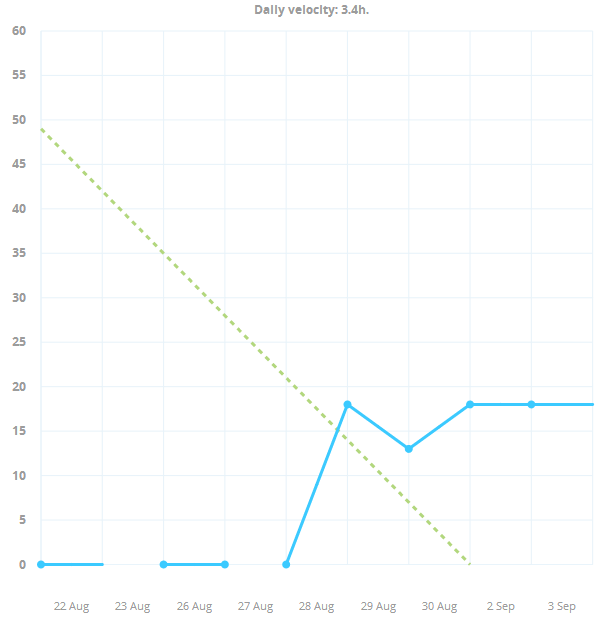
\includegraphics[width=10cm]{sprint0/burn_down_sprint0.png}
%	\caption{Sprint0 Burn Down Chart}
%	\label{fig:sprint0_burn_down_chart}
%\end{figure}


\section{Architecture}
\section{Implementation}
\section{Testing}
\section{Occurring risks}
\section{Retrospective}
\subsection{Pros}
\subsection{Cons}
\section{Evaluation}



\subsubsection{Sprint 0 [probably delete]}
We have embraced Sprint 0 as a preliminary sprint, when we can set up all necessary collaboration tools, equipment, prepare templates for meetings and mainly to acquaint ourselves with Scrum methodology. The original plan was to finish sprint 0 on 8th of September, but we have decided to terminate it prematurely due to finishing sprint goals in shorter time than we had expected. Other reason for terminating the sprint was desire to start actually working on the product itself.

\paragraph{Sprint goals:}
\begin{itemize}
    \item Read compendium
    \item Find and agree suitable collaboration tools
    \item Start working the Project plan
    \item Fill backlog with stories
    \item Assign roles to members of the team
    \item Assign a name to our project
\end{itemize}